\documentclass{article}
\usepackage[T1]{fontenc}

\usepackage{graphicx}
\usepackage{listings}
\begin{document}

\title{FOSS Lab Report}
\author{Gokul K\\[2\baselineskip]
Roll Number: 21\\[2\baselineskip]}
\date{06 February 2020}

\maketitle

\setcounter{section}{18}
\section{Perl Scripting}
\subsection{Aim}
Create a text file and answer the following queries:\newline
	a) Search for the pattern ‘apple’ in the file and display
  the number of occurences.\newline
	b) Count the number of words that ends with ‘e’\newline
	c) Count the number of words that starts with ‘ap’\newline
	d) Search for words containing ‘a’ or ‘s’\newline
	e) Search for words containing zero or more occurrence of ‘e’\newline
	f) Search for words containing one or more occurrence of ‘e’\newline
	g) Search for words containing the letters ‘l’ and ‘m’, with 
	any number of characters in between.

\subsection{Source Code}
\begin{verbatim}
    #! /usr/bin/env perl
    
    # Create a text file and answer the following queries :
    # 	a) Search for the pattern ‘apple’ in the file and display
    #   the number of occurences.
    # 	b) Count the number of words that ends with ‘e’
    # 	c) Count the number of words that starts with ‘ap’
    # 	d) Search for words containing ‘a’ or ‘s’
    # 	e) Search for words containing zero or more occurrence of ‘e’
    # 	f) Search for words containing one or more occurrence of ‘e’
    # 	g) Search for words containing the letters ‘l’ and ‘m’, with 
    # 	any number of characters in between.
    
    
    use strict;
    use warnings;
      
    open my $file, "<", "data.txt" or die "Couldnt find file data.txt";  
    
    my $apple = 0;
    my $e = 0;
    my $ap = 0;
    my $as = 0;
    
    while(<$file>) {
        my $line = $_;
        my @arr = split /\s+/, $line;
        for my $word (@arr) {
                    $apple += () = $word =~ m\apple\gi;
            $e += () = $word =~ m\.*e$\gi;
            $ap += () = $word =~ m\^ap\gi;
        }
    }
    
    print "Number of occurences of apple: $apple\n";
    print "Number of words that ends with e: $e\n";
    print "Number of words that ends with ap: $ap\n";
    
    seek $file, 0, 0;
    print "\nWords with either a or s:\n";
    while(<$file>) {
            my $line = $_;
            my @arr = split /\s+/, $line;
            for my $word (@arr) {
                    if($word =~ m\.*[as].*\){
                            print "$&\n";
                    }
            }
    }
    
    seek $file, 0, 0;
    print "\nWords containing 0 or more e:\n";
    while(<$file>) {
            my $line = $_;
            my @arr = split /\s+/, $line;
            for my $word (@arr) {
                    if($word =~ m\.*e?.*\){
                            print "$&\n";
                    }
            }
    }
    
    seek $file, 0, 0;
    print "\nWords containing 1 or more e:\n";
    while(<$file>) {
            my $line = $_;
            my @arr = split /\s+/, $line;
            for my $word (@arr) {
                    if($word =~ m\.*e.*\){
                            print "$&\n";
                    }
            }
    }
    
    seek $file, 0, 0;
    print "\nWords with l & m and characters in between:\n";
    while(<$file>) {
            my $line = $_;
            my @arr = split /\s+/, $line;
            for my $word (@arr) {
                    if($word =~ m\.*l.*m.*\){
                            print "$&\n";
                    }
            }
    }
    close($file);
\end{verbatim}

\subsection{Program Description}
Perl is a programming language developed by Larry Wall, especially designed
for text processing. It stands for Practical Extraction and Report Language.
It runs on a variety of platforms, such as Windows, Mac OS, and the 
various versions of UNIX. This tutorial provides a complete understanding
on Perl\newline
The given text files is splitted in to each words using regular expression
pattern matching. Then each queries are conducted by building corresponding
RegEx and matching it with each word in the file.

\subsection{Output}
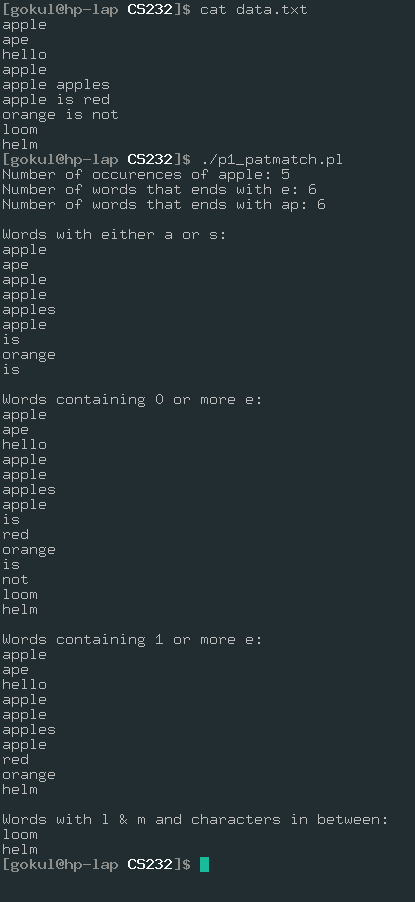
\includegraphics[width=0.9\textwidth]{img/p19.png}\newline

\subsection{Result}
The above program is run on Manjaro Linux running perl 5, version 30. 
Each query is checked and output is verified
\end{document}